\newpage
\section{Suggested solutions: Infinite Impulse Response Filters}

\begin{enumerate}
\item Let $y[n]=\mathcal{T}\{x[n]\}$ be a discrete LTI system, defined as:
$$y[n]=y[n-1]+y[n-2]+x[n-1].$$

\begin{enumerate}[a)]
\item The impulse response is simply $h[n]=\mathcal{T}\{\delta[n]\}$, giving that $h[n]$ must satisfy the following difference equation:
$$h[n]=h[n-1]+h[n-2]+\delta[n-1].$$
Assume $h[n]=0$ for $n<0$, then by iterating, we have:
\begin{align*}
    h[0]&= h[-1] + h[-2] + \delta[0-1]=0, \\
    h[1]&= h[0]  + h[-1] + \delta[0]=1, \\
    h[2]&= h[1]  + h[0]  + \delta[1]=1, \\
    h[3]&= h[2]  + h[1]  + \delta[2]=2, \\
    h[4]&= h[3]  + h[2]  + \delta[3]=3, \\
    h[5]&= h[4]  + h[2]  + \delta[4]=5, 
\end{align*}
as we wanted to show.

\item This is an infinite impulse response filter as it can be written as:
$$y[n]=\sum_{l=1}^{2} a_{l}y[n-l]+\sum_{k=0}^{1} b_{k}x[n-l],$$
with $a_{1}=a_{2}=1$, $b_{0}=0$ and $b_{1}=1$. 

\item Calculating the $z$-transform, one gets
\begin{align*}
    Y(z)&=\mathcal{Z}\{y[n]\}=\mathcal{Z}\{y[n-1]\}+\mathcal{Z}\{y[n-2]\}+\mathcal{Z}\{x[n-1]\}, \\
    Y(z)&=z^{-1}\mathcal{Z}\{y[n]\} + z^{-2}\mathcal{Z}\{y[n]\} + z^{-1}\mathcal{Z}\{x[n]\}, \\
    Y(z)&=z^{-1}Y(z) + z^{-2}Y(z) + z^{-1}X(z),
\end{align*}
where the final equation can be solved to obtain:
$$Y(z)=\frac{z^{-1}X(z)}{1-z^{-1}-z^{-2}}.$$

\item The system function is, by definition, the function $\mathcal{H}(z)$, such that:
$$Y(z)=\mathcal{H}(z)X(z).$$
Clearly, we must have:
$$\mathcal{H}(z)=\frac{z^{-1}}{1-z^{-1}-z^{-2}}.$$
This can be factored as:
$$\mathcal{H}(z)=\frac{z^{-1}}{(1-\varphi_{1}z^{-1})(1-\varphi_{2}z^{-1})},$$
where $\varphi_{1}$ and $\varphi_{2}$ are the roots of the quadratic equation:
$$z^{2}-z-1=0.$$

\item The values of $\varphi_{1}$ and $\varphi_{2}$ are the roots of the equation $z^{2}-z-1$. You can easily find the roots by solving the quadratic equation by the standard formula. On the other, the equation is the second degree polynomial that defined the golden ratio, therefore, we know the roots are:
\begin{align*}
    \varphi_{1} &= \frac{1+\sqrt{5}}{2}, \\
    \varphi_{2} &= \frac{1-\sqrt{5}}{2}.
\end{align*}

\item Apply partial fraction decomposition to the system function:
$$\mathcal{H}(z)=\frac{z^{-1}}{(1-\varphi_{1}z^{-1})(1-\varphi_{2}z^{-1})}=\frac{A}{1-\varphi_{1}z^{-1}}+\frac{B}{1-\varphi_{2}z^{-1}},$$
from which we get:
$$z^{-1}=A(1-\varphi_{2}z^{-1})+B(1-\varphi_{1}z^{-1}).$$
Collecting terms gives the following relations:
\begin{align*}
    A + B &= 0, \\
    -A\varphi_{2}-B\varphi_{1} &= 1.
\end{align*}
Solving this linear system, we conclude that:
\begin{align*}
    A &= \frac{1}{\varphi_{1}-\varphi_{2}}, \\
    B &= -\frac{1}{\varphi_{1}-\varphi_{2}}.
\end{align*}
The system function can then be written as:
$$\mathcal{H}(z)=\frac{1}{\varphi_{1}-\varphi_{2}}\frac{1}{1-\varphi_{1}z^{-1}}-\frac{1}{\varphi_{1}-\varphi_{2}}\frac{1}{1-\varphi_{2}z^{-1}}.$$
Apply the inverse $z$-transform:
\begin{align*}
    h[n]&=\mathcal{Z}^{-1}\{\mathcal{H}(z)\}=\frac{1}{\varphi_{1}-\varphi_{2}}\mathcal{Z}^{-1}\left\{\frac{1}{1-\varphi_{1}z^{-1}}\right\}-\frac{1}{\varphi_{1}-\varphi_{2}}\mathcal{Z}^{-1}\left\{\frac{1}{1-\varphi_{2}z^{-1}}\right\}, \\
    &=\frac{1}{\varphi_{1}-\varphi_{2}}\varphi_{1}^{n}u[n] - \frac{1}{\varphi_{1}-\varphi_{2}}\varphi_{2}^{n}u[n].
\end{align*}
You can verify that this is indeed a function that generates the Fibonacci sequence (do it!).

\item Let $x[n]$ be bounded, that is, $x[n]$ shall satisfy:
$$|x[n]|\le M_{x},$$
for all $n$, for some finite number $M_{x}<\infty$. For any LTI system, a sufficient condition for the system to be BIBO is that the impulse response function is bounded, thus we must have:
$$\sum_{k=-\infty}^{\infty}|h[k]|\le M_{h},$$
for some $M_{h}<\infty$. This gives that:
$$\sum_{k=-\infty}^{\infty}\left|\frac{\varphi_{1}^{k}-\varphi_{2}^{k}}{\varphi_{1}-\varphi_{2}}\right|=\frac{1}{|\varphi_{1}-\varphi_{2}|}\sum_{k=-\infty}^{\infty}|\varphi_{1}^{k}-\varphi_{2}^{k}|.$$
This series diverges, hence the system is not BIBO. 

\end{enumerate}

\item If a time-shifted unit impulse: $x[n]=\delta[n-n_0]$ satisfy $X(z)=z^{-n_{0}}$. Then the discrete-time Fourier transform is the $z$-transform evaluated on the unit circle. Thus:
$$\mathcal{F}\{x[n]\}=\mathcal{Z}\{x[n]\}|_{z=e^{i\hat{\omega}}}=(e^{i\hat{\omega}})^{-n_{0}}=e^{-i\hat{\omega}n_{0}}.$$
You can compare this with previous results and see that it is correct. 

\item Recall that the following inverse $z$-transforms:
\begin{align*}
    \mathcal{Z}^{-1}\{z^{-k}\}&= \delta[n-k], \\
    \mathcal{Z}^{-1}\left\{\frac{b}{1-az^{-1}}\right\}&=ba^{n}u[n].
\end{align*}
\begin{enumerate}[a)]
\item For the complex function:
$$A(z)=\frac{1+2z^{-2}}{1-0.25z^{-1}},$$
we can apply polynomial division to obtain:
$$A(z)=-8z^{-1}-32+\frac{33}{1-0.25z^{-1}}.$$
Now $A(z)$ consists of known inverse $z$-transforms. The inverse $z$-transform of $A(z)$ is then:
$$a[n]=\mathcal{Z}^{-1}\{A(z)\}=\underline{\underline{-8\delta[n-1]-32\delta[n]+33(0.25)^{n}u[n]}}.$$

\item For the complex function:
$$B(z)=\frac{3}{1-0.3z^{-1}}-\frac{2}{1+0.7z^{-1}},$$
we can apply the known inverse $z$-transforms immediately:
$$b[n]=\mathcal{Z}^{-1}\{B(z)\}=\underline{\underline{3(0.3)^{n}u[n]-2(-0.7)^{n}u[n]}}.$$

\item For the complex function: 
$$C(z)=\frac{1+2z^{-2}}{1-0.4z^{-1}-0.32z^{-2}},$$
we apply a polynomial division:
$$C(z)=-6.25+\frac{7.25-2.5z^{-1}}{1-0.4z^{-1}-0.32z^{-2}}.$$
Factor the denominator:
$$C(z)=-6.25+\frac{7.25-2.5z^{-1}}{0.32(2.5+z^{-1})(1.25-z^{-1})}.$$
Apply a partial fraction decomposition on the last term:
\begin{align*}
    \frac{7.25-2.5z^{-1}}{0.32(2.5+z^{-1})(1.25-z^{-1})}&=\frac{A}{2.5+z^{-1}}+\frac{B}{1.25-z^{-1}}, \\
    7.25-2.5z^{-1}&=0.32A(1.25-z^{-1}) + 0.32B(2.5+z^{-1}).
\end{align*}
Get the following linear relations:
\begin{align*}
    (0.32)(1.25)A + (0.32)(2.5)B &= 7.25, \\
    -0.32A + 0.32B &= -2.5,
\end{align*}
so $A=11.25$ and $B=3.4375$. Then $C(z)$ can be written as:
\begin{align*}
    C(z)&=-6.25+\frac{11.25}{2.5+z^{-1}}+\frac{3.4375}{1.25-z^{-1}}, \\
    &=-6.25 + \frac{4.5}{1+0.4z^{-1}} + \frac{2.75}{1-0.8z^{-1}}.
\end{align*}
Now, we can apply our known inverse $z$-transform pairs to obtain:
$$\underline{\underline{c[n]=-6.25\delta[n]+4.5(-0.4)^{n}u[n]+2.75(0.8)^{n}u[n]}}.$$
\end{enumerate}

\item Let $y[n]$ be given by the difference equation:
$$y[n]=0.8y[n-1]+5x[n].$$

\begin{enumerate}[a)]
\item The equation contains $y[n-1]$ depending on one past value, hence the filter is an IIR.

\item To find the system function, apply the $z$-transform:
$$Y(z)=0.8z^{-1}Y(z)+5X(z),$$
where $Y(z)=\mathcal{Z}\{y[n]\}$ and $X(z)=\mathcal{Z}\{x[n]\}$. Rewriting it on the form $Y(z)=\mathcal{H}(z)X(z)$ one gets:
$$Y(z)=\frac{5}{1-0.8z^{-1}}X(z),$$
so the system function is:
$$\mathcal{H}(z)=\frac{5}{1-0.8z^{-1}}.$$

\item A pole-zero diagram for this system is shown in Figure \ref{iir:ex3}.
\begin{marginfigure}[-5cm]
\begin{center}
\begin{tikzpicture}
	\begin{axis}[axis equal, ymin=-1.5,xmin=-1.5,ymax=1.5,xmax=1.5,  ticks=none,
    xlabel=$\mathrm{Re}(z)$,
    ylabel=$\mathrm{Im}(z)$, axis lines = middle, width=7cm, height=7cm]
	\addplot [gray,domain=0:2*pi,samples=50]({cos(deg(x))},{sin(deg(x))});
\addplot [red, mark = x,mark size=3pt] coordinates {({0}, {0})} {}; 
\addplot [red, mark = x, mark size=3pt] coordinates {(0.8,0)};
\end{axis}
\end{tikzpicture}
\end{center}
\caption{The system function has no zeros in this case. There are two poles, these being at $z=0$ and at $z=0.8$, both marked with red crosses.}
\label{iir:ex3}
\end{marginfigure}

The poles for this system function all lie inside the unit circle, so the system is stable. 

\item The impulse response function can be found by the inverse $z$-transform of the system function. In this case, we get:
$$h[n]=\mathcal{Z}^{-1}\left\{\mathcal{H}(z)\right\}=\mathcal{Z}^{-1}\left\{\frac{5}{1-0.8z^{-1}}\right\}=5(0.8)^{n}u[n].$$

\item Any discrete LTI system can be written on the form: $$y[n]=|\mathcal{H}(\hat{\omega})|\angle\mathcal{H}(\hat{\omega}) x[n],$$
so the frequencies are multiplied with $|\mathcal{H}(\hat{\omega})|$. In this case, the filter is a low-pass filter. This can be seen by drawing the magnitude response function, $|\mathcal{H}(\hat{\omega})|$. Low frequencies are attenuated while high frequencies are reduced, signifying a low-pass filter. 

\item The filter is LTI, so the system can be written as a convolution:
$$y[n]=h[n]*x[n].$$
Taking $x[n]=u[n]$ gives:
\begin{align*}
    y[n] &= h[n]*u[n] = \sum_{k=-\infty}^{\infty}u[k]h[n-k] = \sum_{k=0}^{\infty}h[n-k]. 
\end{align*}
Set $m=n-k$, then the series can be rewritten as:
\begin{align*}
    y[n] &= \sum_{m=-\infty}^{n}h[m], \\
         &= \sum_{m=-\infty}^{n}5(0.8)^{m}u[m],
\end{align*}
now $u[m]$ kills the negative terms as $u[m]=0$ for $m<0$ and $u[m]=1$ for $m\ge 1$, thus the series simplifies to a regular sum, which can be found by the formula for a geometric sum:
\begin{align*}
    y[n] &= 5\sum_{m=0}^{n}(0.8)^{m}, \\
    &= 5\frac{1-0.8^{n+1}}{1-0.8} = 25(1-0.8^{n+1}).
\end{align*}
\end{enumerate}

\item Consider the diagrams in Figure \ref{fig:exzone}.
\begin{enumerate}[a)]
\item The first diagram has a pole at $0$ and three zeros. There is a zero at $z=1$, which corresponds to $\hat{\omega}=0$, thus this frequency is filtered out. The other zeros and poles are barely noticeable, but the function will dip close to the zeros. For diagram b) there is a pole at $z=1$, which is on the unit circle. Therefore, the function will tend towards infinity here. The other poles don't do much in comparison, but some small peaks would occur at these values. The last diagram filters out $\hat{\omega}=\pm\pi$ as there is a zero for $z=-1$. A plot of the magnitude responses is shown in Figure \ref{fig:mag_res_diag}.

\begin{figure}
    \centering
    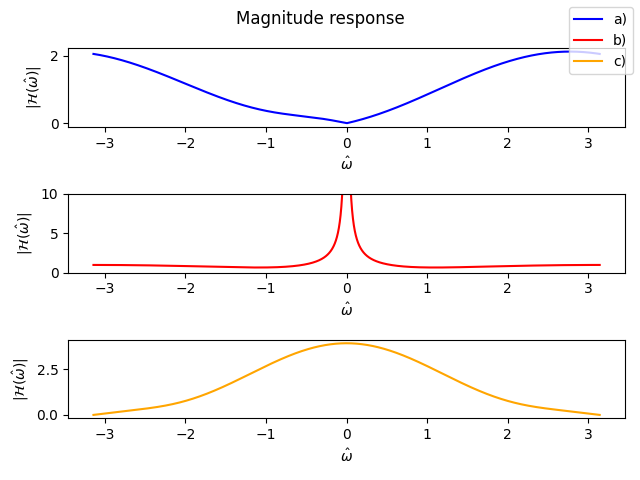
\includegraphics[width=10.5cm,height=8.0cm]{ch19/figures/magn_resp_diag.png}
    \caption{Magnitude response for the three pole-zero diagrams. Note that the limits of b) has been set to 0-10.}
    \label{fig:mag_res_diag}
\end{figure}

\item The system function:
$$\mathcal{H}(z)=\frac{(z+1)(z-\alpha)(z-\alpha^{*})}{z^{3}}$$
has zeros corresponding to $z=-1,\alpha,\alpha^{*}$, thus this is the system function corresponding to diagram c) as $\alpha=i(2\sqrt{2})^{-1}-(2\sqrt{2})^{-1}$, which has a negative real part. 
\item Diagram b) and c) both reduce high frequency components and keeps low frequency components, meaning both of these are low-pass filters. However, only diagram c) is stable. This can be seen from Figure \ref{fig:mag_res_diag} as the magnitude response becomes unbounded at $\hat{\omega}=0$, but we can also see this from the pole-zero diagram, as diagram b) has a pole on the unit circle. Recall that a system function corresponds to a stable BIBO LTI system if all the poles lie inside the unit circle. 

\item The only diagram left is a), as b) and c) are both low-pass filters. Diagram a) is indeed a high-pass filter as $\hat{\omega}=0$ gets sent to $0$ and the high frequencies pass through. The filter is also stable as all the poles lie inside the unit circle. 

\item The filter corresponding to diagram c) filters out $\hat{\omega}=\pi$ completely. 

\item Diagram a) and diagram c) represents a FIR filter, as these only have a pole at $0$. Recall that the system function for a 
FIR filter can be found by feeding a $\delta[n]$ into the LTI system. Observe:
$$y[n]=\sum_k b_kx[n-k],$$
which yield a system function of the form:
$$\mathcal{H}(z)=\sum b_{k}z^{-k}.$$

\end{enumerate}
\end{enumerate}